%%%%%%%%%%%%2019.3.12第三周Mon%%%%%%%%%%%%%%%%%%%%%%%
%%%%%%%%%%%%%%%%下周一,周坚代课%%&%%%%%%%%%%%%%%%%%%
%%%%%%%%%%%%%%%%下周二,随堂考试%%%%%%%%%%%%%%%%%%%%%

%\textbf{Coalgebra and homotopy associativity}



\chapter{形变量子化}

%%%%%%%%%%2019.3.18第四周 周一%%%%%%%%%%%%%%%%%%%%%%%
%%%%%%%%%%%%%%%%李思出差,别人代课%%%%%%%%%%%%%%%%%%%
本章开始,正式搞一些事情。
经典力学与量子力学的框架众所周知,大致如下:

\index{phase space\kong 相空间}
\index{symplectic manifold\kong 辛流形}
\index{observable\kong 观测量}
\index{Hamiltonian\kong 哈密顿量}

$$
  \begin{tabular}{|c|c|c|}
    \hline
             &经典力学 &量子力学\\
    \hline
    相空间   &辛流形$(X,\omg)$   &希尔伯特空间$\mcalH$\\
    观测量   &光滑函数           &厄密特算子  \\
    演化方程 &$\frac{\td f}{\td t}=\{H,f\}$
    &$\frac{\td A_t}{\td t}=\frac{i}{\hbar}[\hat{H},A_t]$\\
    \hline
  \end{tabular}
$$

我们将利用结合代数的Hochschild(上)同调,以及$A_{\infty}$方法,
来证明Kontsevich的Formality theorem.

{\color{red}(待完善)}

%\textbf{Poisson structure and quantization}

%Motiration
%Classical Mechanics
%Phase space$(X,\omg)\rightsquigarrow$ Sympletic mfd
%observables: $C^{\infty}(X)$: smooth function
%Poisson bracket:
%$C^{\infty}(X)\ten X^{\infty}(X)\to C^{\infty}(X)$
%Dynamics - Hamiltionian function $H\in C^{\infty}(X)$
%s.t. $\frac{\td f}{\td t}=\{H,f\}$.

%Quantum Picture:
%Hilbert space
%$$\frac{\td A_t}{\td t}=\frac{i}{\hbar}[\hat{H},A_t]$$
%Associative algebra.
%$A_{\infty}$-method and Hochcshild homology
%\textbf{Goal: Formality thm(Kontsevich)}
%Now, let us begin...
%\vs

\section{泊松几何与辛几何}
%\textbf{Poisson bracket}

本节简要回顾一下泊松几何。

\begin{definition}(泊松括号)
\index{Poisson bracket\kong 泊松括号}
%let $X$ be a smooth manifold, a Poisson bracket
%on $C^{\infty}(X)$ is  a $\bbR$-linear
%$$\{,\}:C^{\infty}(X)\times C^{\infty}(X)\to C^{\infty}(X)$$
%sarisfies
%skew symmetry
%Leibnitz rule
%Jacobi identity

设$X$为光滑流形,$\{,\}:C^{\infty}(X)\times C^{\infty}(X)\to C^{\infty}(X)$
为$\bbR$-双线性映射。称$\{,\}$为$X$上的\textbf{泊松括号}(Poisson bracket),
如果$\{,\}$满足:
对任意$f,g,h\in C^{\infty}(X)$,成立

(1)反对称性:$$\{f,g\}=-\{g,f\}$$

(2)Jacobi恒等式:
$$\{f,\{g,h\}\}+\{g,\{h,f\}\}+\{h,\{f,g\}\}=0$$

(3)Leibnitz法则:
$$\{f,gh\}=\{f,g\}h+g\{f,h\}$$
\end{definition}


泊松括号的定义的(1)(2)表明$(C^{\infty}(X),\{,\})$为李代数,
而(3)表明对任意$f\in C^{\infty}(X)$,映射
\begin{eqnarray*}
X_f:C^{\infty}(X)&\to& C^{\infty}(X)\\
g &\mapsto& \{f,g\}
\end{eqnarray*}
为导子,从而$X_f$为$X$上的光滑切向量场,
在局部坐标下形如$X_f=X_f^i\pp{u^i}$.于是有
$$\{f,g\}=X_f^i\pfrac{g}{u^i}$$
但又注意到$\{f,g\}=-\{g,f\}$以及切向量场$X_g$,
从而易知泊松括号$\{,\}$在局部坐标$(u^i)$下的表达式必形如
$$\{f,g\}=P^{ij}\pfrac{f}{u^i}\pfrac{g}{u^j}$$
并且容易验证:
\begin{lemma}设$\{,\}$为光滑流形$X$上的泊松括号,
并且在局部坐标$(u^i)$下的表达式为
$$\{f,g\}=P^{ij}\pfrac{f}{u^i}\pfrac{g}{u^j}$$
那么对任意指标$i,j,k$,成立
$$P^{ij}=-P^{ji}$$
$$P^{is}\pfrac{P^{jk}}{u^s}+
P^{js}\pfrac{P^{ki}}{u^s}+
P^{ks}\pfrac{P^{ij}}{u^s}=0$$
\end{lemma}

\begin{proof}
容易验证$P^{ij}=-P^{ji}$等价于泊松括号的反对称性$\{f,g\}=-\{g,f\}$,
这是因为对任意光滑函数$f,g$,局部上有
$$P^{ij}\pfrac{f}{u^i}\pfrac{g}{u^j}=\{f,g\}=-\{g,f\}
=-P^{ij}\pfrac{g}{u^i}\pfrac{f}{u^j}=
-P^{ji}\pfrac{f}{u^i}\pfrac{g}{u^j}$$
从而$(P^{ij}+P^{ji})\pfrac{f}{u^i}\pfrac{g}{u^j}=0$,
因此由$f,g$的任意性,有$P^{ij}=-P^{ji}$.\vs

再看第二个式子。事实上它等价于泊松括号的雅可比恒等式。
对任意$f,g,h\in C^{\infty}(X)$,局部坐标下有
\begin{eqnarray*}
     \{f,\{g,h\}\}
&=&
     \{f,P^{ij}\pfrac{g}{u^i}\pfrac{h}{u^j}\}\\
&=&
     P^{kl}\pfrac{f}{u^k}
     \pfrac{P^{ij}}{u^l}
     \pfrac{g}{u^i}
     \pfrac{h}{u^j}
    +P^{ij}P^{kl}\pfrac{f}{u^k}
     \left(
       \pmfrac{g}{u^i}{u^l}\pfrac{h}{u^j}
      +\pmfrac{h}{u^j}{u^l}\pfrac{g}{u^i}
     \right)
\end{eqnarray*}
将$f,g,h$轮换再相加,适当更改求和指标,合并整理得
\begin{eqnarray*}
& &
     \{f,\{g,h\}\}+\{g,\{h,f\}\}+\{h,\{f,g\}\}\\
&=&
     \pfrac{f}{u^i}
     \pfrac{g}{u^j}
     \pfrac{h}{u^k}
     \left(
       P^{is}\pfrac{P^{jk}}{u^s}
      +P^{js}\pfrac{P^{ki}}{u^s}
      +P^{ks}\pfrac{P^{ij}}{u^s}
     \right)
    +P^{kl}(P^{ij}+P^{ji})
     \pfrac{f}{u^k}
     \pmfrac{g}{u^i}{u^l}
     \pfrac{h}{u^j}\\
& &
    +P^{kl}(P^{ij}+P^{ji})
     \pfrac{g}{u^k}
     \pmfrac{h}{u^i}{u^l}
     \pfrac{f}{u^j}
    +P^{kl}(P^{ij}+P^{ji})
     \pfrac{h}{u^k}
     \pmfrac{f}{u^i}{u^l}
     \pfrac{g}{u^j}
\end{eqnarray*}
注意到$P^{ij}=-P^{ji}$,以及$f,g,h$的任意性,从而有
$$
 P^{is}\pfrac{P^{jk}}{u^s}
+P^{js}\pfrac{P^{ki}}{u^s}
+P^{ks}\pfrac{P^{ij}}{u^s}
=0
$$
得证。
\end{proof}

我们可以使用张量的语言来描述泊松括号结构:

\begin{definition}(泊松张量)
对于光滑流形$X$,以及$P\in\PV^2_X$为$2$-切向量场,
在局部坐标下表达式为
$$P=P^{ij}\pp{u^i}\wedge\pp{u^j}$$
其中$P^{ij}=-P^{ji}$.称$P$为\textbf{泊松张量}(Poisson tensor),
\index{Poisson tensor\kong 泊松张量}
如果$P$在局部坐标下满足如下雅可比恒等式:
$$
 P^{is}\pfrac{P^{jk}}{u^s}
+P^{js}\pfrac{P^{ki}}{u^s}
+P^{ks}\pfrac{P^{ij}}{u^s}
=0
$$
\end{definition}
容易看出泊松括号与泊松张量的一一对应关系:
对于泊松括号$\{,\}$,若局部上有
$\{f,g\}=P^{ij}\pfrac{f}{u^i}\pfrac{g}{u^j}$,
则考虑泊松张量
$$P:=\frac{1}{2}P^{ij}\pp{u^i}\wedge\pp{u^j}$$
反过来,由泊松张量也能得到泊松括号。并且容易知道
$$\{f,g\}=\langle P,\td f\wedge\td g\rangle$$

%Poisson tensor:
%$P\in\Gamma(X,\wedgeform{2}TX)=\PV_X^2$ s.t.
%$$\{f,g\}=\langle P, \td f\wedge \td g\rangle$$
%$$=P^{ij}(\p_i f\p_jg-\p_ig\p_jf)$$

%Check: Jacobi identity $\iff[P,P]=0$, where
%$[,]$ is Schouten-Nijenhuis bracket.

事实上泊松张量的雅可比恒等式可以用Schouten-Nijenhuis括号等价刻画:

\begin{prop}对于光滑流形$X$,以及$P\in\PV^2_X$,
则$P$为泊松张量当且仅当
$$[P,P]=0$$
其中$[,]$为Schouten-Nijenhuis括号
(见定义\ref{Schouten-Nijenhuis定义-def})。
\end{prop}

\begin{proof}
局部坐标下验证。取局部坐标$(u^i)$,
令$P=P^{ij}\pp{u^i}\wedge\pp{u^j}$,则有
\begin{eqnarray*}
     [P,P]
&=&
     \big[(P^{ij}\pp{u^i})\wedge\pp{u^j},
     (P^{kl}\pp{u^k})\wedge\pp{u^l}\big]\\
&=&
     [P^{ij}\pp{u^i},P^{kl}\pp{u^k}]\wedge\pp{u^j}\wedge\pp{u^l}
    -[P^{ij}\pp{u^i},\pp{u^l}]\wedge\pp{u^j}\wedge P^{kl}\pp{u^k}\\
& &
    -[\pp{u^j},P^{kl}\pp{u^k}]\wedge P^{ij}\pp{u^i}\wedge\pp{u^l}
    +[\pp{u^j},\pp{u^l}]\wedge P^{ij}\pp{u^i}\wedge P^{kl}\pp{u^k}
\end{eqnarray*}
上式右端共有四项,首先注意最后一项
$$[\pp{u^j},\pp{u^l}]\wedge P^{ij}\pp{u^i}\wedge P^{kl}\pp{u^k}
=P^{ij}P^{kl}\delta_{jl}\pp{u^j}\wedge\pp{u^i}\wedge\pp{u^k}
=\sum_{j=1}^nP^{ij}P^{kj}
 \pp{u^j}\wedge\pp{u^i}\wedge\pp{u^k}=0$$
最后一个等号是因为指标$i,k$的(反)对称性;
从而暴力展开,注意利用$P^{ij}=-P^{ji}$以及适当更改求和指标,有
\begin{eqnarray*}
     [P,P]
&=&
     [P^{ij}\pp{u^i},P^{kl}\pp{u^k}]\wedge\pp{u^j}\wedge\pp{u^l}\\
& &
    -[P^{ij}\pp{u^i},\pp{u^l}]\wedge\pp{u^j}\wedge P^{kl}\pp{u^k}
    -[\pp{u^j},P^{kl}\pp{u^k}]\wedge P^{ij}\pp{u^i}\wedge\pp{u^l}\\
&=&
     P^{ij}\pfrac{P^{kl}}{u^i}
     \pp{u^k}\wedge\pp{u^j}\wedge\pp{u^l}
    -P^{kl}\pfrac{P^{ij}}{u^k}
     \pp{u^i}\wedge\pp{u^j}\wedge\pp{u^l}\\
& &
    +P^{kl}\pfrac{P^{ij}}{u^l}
     \pp{u^i}\wedge\pp{u^j}\wedge\pp{u^k}
    -P^{ij}\pfrac{P^{kl}}{u^j}
     \pp{u^k}\wedge\pp{u^i}\wedge\pp{u^l}\\
&=&
     \left(
       -P^{sj}\pfrac{P^{ki}}{u^s}
       -P^{sk}\pfrac{P^{ij}}{u^s}
       +P^{ks}\pfrac{P^{ij}}{u^s}
       -P^{js}\pfrac{P^{ik}}{u^s}
     \right)
     \pp{u^i}\wedge\pp{u^j}\wedge\pp{u^k}\\
&=&
     -4P^{sj}\pfrac{P^{ki}}{u^s}
     \pp{u^i}\wedge\pp{u^j}\wedge\pp{u^k}\\
&=&
     -8\sum_{i<j<k}
       \left(
          P^{sj}\pfrac{P^{ki}}{u^s}
         +P^{sk}\pfrac{P^{ij}}{u^s}
         +P^{si}\pfrac{P^{jk}}{u^s}
       \right)
     \pp{u^i}\wedge\pp{u^j}\wedge\pp{u^k}
\end{eqnarray*}
可见$[P,P]=0$当且仅当雅可比恒等式成立,证毕。
\end{proof}

于是我们自然地引入泊松流形的概念:

\begin{definition}(泊松流形)
\index{Poisson manifold\kong 泊松流形}

\textbf{泊松流形}(Poisson manifold)
是指二元组$(X,P)$,其中$X$为光滑流形,
$P\in\PV^2_X$满足$[P,P]=0$.
%A Poisson manifold is a pair $(X,P)$ such that
%$[P,P]=0$ for some $P\in\PV_X^2$.
\end{definition}
众所周知,这是经典力学的几何模型。
%(geometry of classical mechanics)
接下来看一些泊松流形的例子:

\begin{Example}(由辛结构诱导的泊松结构)
%if $(X,\omg)$ is a sympletic manifold,

设$(X,\omg)$为辛流形,其中辛形式
$$\omg=\frac{1}{2}\omg_{ij}\td x^i\wedge\td x^{j}$$
满足$\td\omg=0$,并且使得系数矩阵
$(\omg_{ij})_{1\leq i,j\leq n}$在$X$上处处可逆、反对称。
那么辛结构$\omg$自然诱导泊松结构
%such that $\omg$ is non-degenerated ,$\omg_{ij}=-\omg_{ji}$,
%then
$$\omg^{-1}:=\frac{1}{2}\omg^{ij}\p_i\wedge\p_j$$
其中矩阵$(\omg^{ij}):=(\omg_{ij})^{-1}$.
%is a Poisson bracket.where $(\omg^{ij}):=(\omg_{ij})^{-1}$
\end{Example}

\begin{proof}
我们只需验证雅可比恒等式
$$
  \omg^{is}\pfrac{\omg^{jk}}{u^s}
 +\omg^{js}\pfrac{\omg^{ki}}{u^s}
 +\omg^{ks}\pfrac{\omg^{ij}}{u^s}
=0
$$

一方面注意到逆矩阵求导公式
$\pfrac{\omg^{-1}}{u^s}=
-\omg^{-1}\pfrac{\omg}{u^s}\omg^{-1}$,从而有
$$\omg^{is}\pfrac{\omg^{jk}}{u^s}=-
\omg^{is}\omg^{jm}\omg^{nk}\pfrac{\omg_{mn}}{u^s}$$
对$i,j,k$轮换求和,有
$$
  \omg^{is}\pfrac{\omg^{jk}}{u^s}
 +\omg^{js}\pfrac{\omg^{ki}}{u^s}
 +\omg^{ks}\pfrac{\omg^{ij}}{u^s}
=
  \omg^{is}\omg^{jm}\omg^{kn}
  \left(
    \pfrac{\omg_{mn}}{u^s}
   +\pfrac{\omg_{ns}}{u^m}
   +\pfrac{\omg_{sm}}{u^n}
  \right)
$$

另一方面,由于$\td\omg=0$,从而有
\begin{eqnarray*}
     0
&=&
     \td(\omg_{ij}\td x^i\wedge\td x^j)\\
&=&
     \pfrac{\omg_{ij}}{u^k}\td x^i\wedge\td x^j\wedge\td x^k\\
&=&
     \sum_{i<j<k}
   2\left(
     \pfrac{\omg_{ij}}{u^k}
    +\pfrac{\omg_{jk}}{u^i}
    +\pfrac{\omg_{ki}}{u^j}
   \right)
   \td x^i\wedge\td x^j\wedge\td x^k
\end{eqnarray*}
因此有
$$\pfrac{\omg_{ij}}{u^k}
    +\pfrac{\omg_{jk}}{u^i}
    +\pfrac{\omg_{ki}}{u^j}=0$$

综上两方面,证毕。
\end{proof}
众所周知,这个例子来自经典力学。
事实上,此泊松结构有如下不依赖局部坐标的表达方式:
对任意$f\in C^{\infty}(X)$,存在唯一的切向量场$X_f$使得
$$\td f+i_{X_f}(\omg)=0$$
称此$X_f$为$f$的\textbf{哈密顿向量场}。
于是,对于任意的$f,g\in C^{\infty}(X)$,
辛结构$\omg$诱导的泊松括号满足
$$\{f,g\}=\omg(X_f,X_g)$$
以上是我们在经典力学中熟知的。下一个例子更“接近”经典力学:

\begin{Example}(光滑流形余切丛上的典范辛结构)

设$M$为$n$维光滑流形,$X:=T^*M$为$X$的余切丛,
则定义$X$上的\textbf{典范$1$-形式}$\theta\in\Omg^1_X$为:
$$\theta|_{(\bfx,\bfp)}(\bfv,\xi):=\langle \bfp,\bfv\rangle$$
其中$(\bfx,\bfp)\in X$,
$(\bfv,\xi)\in T_{(\bfx,\bfp)}(X)$,
以及$\bfv\in T_{\bfx}M$.
记$X$上的$2$-形式
$$\omg:=-\td\theta$$
称$\omg$为$T^*M$上的\textbf{典范辛形式}。
\end{Example}

考虑$X=T^*M$的局部坐标$(x^1,x^2,...,x^n;p_1,p_2,...,p_n)$,其中
$x^i$为$M$上的局部坐标。则容易知道典范$1$-形式
$\theta$与典范辛形式$\omg$在该局部坐标下的表达式分别为
$$\theta=\sum_{i=1}^np_i\td x^i$$
$$\omg=\sum_{i=1}^n\td x^i\wedge\td p_i$$

上述$\omg$给出了余切丛$T^*M$的辛流形结构,该辛结构诱导泊松结构,
于是我们可以谈论$X=T^*M$上的泊松括号。

\begin{rem}
记号承上,则存在典范的线性同态
\begin{eqnarray*}
\fai:\Gamma(M,TM)&\to& C^{\infty}(X)\\
\fai(\eta)|_{(\bfx,\bfp)}&=&\langle\bfp,\eta\rangle
\end{eqnarray*}
\label{切向量场视为余切丛上的光滑函数}
\end{rem}

即,通过“非常自然的方式”,将底流形$M$上的切向量场
视为余切丛$X=T^*M$上的光滑函数。该线性同态可以自然延拓到
切丛的对称张量丛的截面上:
$$\fai:\Gamma(M,\Sym(TM))\to C^{\infty}(X)$$
无非是“函数的相乘”而已。

\begin{prop}
设$M$为光滑流形,考虑$X=T^*M$上的典范辛结构,
$\fai:\Gamma(M,TM)\to C^{\infty}(X)$同上,
则对$M$的任意的切向量场$f,g$,成立
$$\fai([f,g])=-\{\fai(f),\fai(g)\}$$
其中左边“$[,]$”为$M$上的切向量场的李括号,
右边$\{,\}$为辛流形$X$上的泊松括号。
\end{prop}

\begin{proof}
局部坐标下验证。取$X$的局部坐标$(x^1,...,x^n;p_1,...,p_n)$,记
$$f=f^i\pp{x^i},\quad g=g^i\pp{x^i}$$
则容易知道
$$\fai(f)=f^i(\bfx)p_i,\quad \fai(g)=g^i(\bfx)p_i$$
注意$X$上的泊松张量
$$P=\pp{x^i}\wedge\pp{p_i}$$
因此有
\begin{eqnarray*}
     \{\fai(f),\fai(g)\}
&=&
     \Langle
       \pp{x^s}\wedge\pp{p_s}
     ,
       \td\fai(f)\wedge\td\fai(g)
     \Rangle\\
&=&
     \left(
       g^s\pfrac{f^i}{x^s}
      -f^s\pfrac{g^i}{x^s}
     \right)
     p_i
\end{eqnarray*}
而另一方面,
$$[f,g]=
\left(
  f^s\pfrac{g^i}{x^s}
 -g^s\pfrac{f^i}{x^s}
\right)\pp{x^i}
\quad\Longrightarrow\quad
\fai([f,g])=
\left(
  f^s\pfrac{g^i}{x^s}
 -g^s\pfrac{f^i}{x^s}
\right)p_i
$$
从而$\fai([f,g])=-\{\fai(f),\fai(g)\}$,得证。
\end{proof}

\section{形变量子化与Moyal星积}
%\textbf{Star product:}
我们开始讨论形变量子化。
{\color{red}(此处应该写几句introduction)}

\begin{definition}(星积)
%A star product $*$ on a Possion mfd $(X,P)$
%is a $\bbR[[\hbar]]$-linear map

对于泊松流形$(X,P)$,称$\bbR[\![\hbar]\!]$-双线性映射
\begin{eqnarray*}
C^{\infty}(X)\fps{\hbar}\times C^{\infty}(X)\fps{\hbar}
&\to& C^{\infty}(X)\fps{\hbar}\\
f\star g&\mapsto& \sum_{k\geq 0}C_k(f,g)\hbar^k
\end{eqnarray*}
为$(X,P)$上的\textbf{星积}(star product),
\index{star product\kong 星积}
%such that:
如果$\star$是结合的,并且对对任意$f,g\in C^{\infty}(X)$,以下成立:

%(1) 乘法$*$是结合的。 %is associative

(1) $\hbar\to 0$时退化为通常的函数乘法:
$$f\star g=fg\mod\hbar$$

(2) $*$的“一阶非交换性”由泊松括号给出:
$$f\star g-g\star f=\hbar\{f,g\}\mod\hbar^2$$
%$$\frac{1}{2}(f*g-g*f)=\hbar\{f,g\}\mod\hbar^2$$
%上一行被注掉的公式为笔记中的原始记载,我怀疑这个公式不对

(3) 对于每个$k\geq 0$,$C_k$为双微分算子:
$$C_k(f,g)=\sum_{\max{\{l,m\}}=k}
C_k^{i_1...i_l;j_1,...,j_m}(\p_{i_1}...\p_{i_l}f)
(\p_{j_1}...\p_{j_m}g)$$
其中系数$C_k^{i_1...i_l;j_1,...,j_m}\in C^{\infty}(X)$.
%, where $C_k^{...}$ is in $C^{\infty}(X)$.
%(bi-differential operator)
%\vs
%then, $(C^{\infty},*)$ is the \textbf{deformation quantization} on $(X,P)$.
\end{definition}

此时,也称$(C^{\infty}(X),\star)$为$(X,P)$的\textbf{形变量子化}
(deformation quantization)。
\index{deformation quantization\kong 形变量子化}

%the first non-commutativity of $*$ is given
%by Poosson bracket.

这里的$\hbar$为形式变元
(物理背景为普朗克常量,这是心照不宣的)。
由定义容易知道,对任意$f\in C^{\infty}(X)$,成立
$$1\star f=f\star 1=f$$
其中$1\in C^{\infty}(X)$为值恒为$1$的常值函数。

此外,容易知道双微分算子
$$C_0(f,g)=fg$$
以及我们不妨
$$C_1(f,g)=\{f,g\}$$

一个基本的问题是,任给一个泊松流形$(X,P)$,
它的形变量子化是否一定存在?答案是肯定的,
Kontsevich用非交换几何的工具给出了证明——这也是我们在后文要详细介绍的。
对于辛流形的特殊情况,形变量子化的存在性相对比较容易证明,
据说辛流形的形变量子化与Atiyah-Singer指标定理有联系。

%(1) Existence of deformations - quantization on any poisson manifolds.
%(Kontsevich's solution using non-commutative method)

%(2) Deformation quantization on symplectic manifold
%$\rightsquigarrow$ Atiyah-Singer index Theorem.

%noncommutative \big/quantum field theory method.

我们先来看一些例子:

%Fundamental Question:
%[Dewilde lemote 1983] for a Poisson manifold, is there $\exists$
%a deformation quantization?
%[Fedosov 1983,1994]

\begin{Example}(Moyal 乘积)
%$(C^{\infty}(X),\{,\})\rightsquigarrow(C^{\infty(X)[[\hbar]]},*)$
%$$X=\bbR^m$$
%Poisson bracket
设$X=\bbR^n$,并配以泊松张量
$$P=P^{ij}\pp{x^i}\wedge\pp{x^j}$$
其中$P^{ij}$皆为常数,则我们定义如下乘积:
对任意$f,g\in C^{\infty}(X)$,
%where $P^{ij}\in\bbR$ are constant.
%then we define
$$(f\star g)(x):=
  \left.
    e^{
        \hbar P^{ij}
        \frac{\p}{\p y_i}
        \frac{\p}{\p z_j}
      }
    f(y)g(z)
  \right|_{y=z=x}$$
则$\star$给出了$(X,P)$的形变量子化。
%%%%%%%此处有图%%%%%55
\index{Moyal product}
\label{Moyal星积-def}
\end{Example}
把算子指数打开,该星积$*$的定义式可以显式地写为
$$
  f\star g
=
  \sum_{k=0}^{\infty}
    \frac{\hbar^k}{k!}
    \sum_{i_1,...,i_k
          \atop
          j_1,...,j_k
         }
      P^{i_1j_1}P^{i_2j_2}\cdots P^{i_kj_k}
      (\p_{i_1}\p_{i_2}\cdots\p_{i_k}f)
      (\p_{j_1}\p_{j_2}\cdots\p_{j_k}g)
$$
容易验证如此定义的$\star$满足
$$f\star g=fg+\frac{\hbar}{2}\{f,g\}+o(\hbar)$$
我们只需要再验证$\star$满足结合律,证明如下:

\begin{proof}直接将$(f\star g)\star h$暴力展开,
对任意$m\geq 0$,计算$\hbar^m$的系数。

为书写方便,引入一些记号:
我们常用$I=(i_1,i_2,...,i_s)$来表示长度为$s$的多重指标,其中
$i_1,...,i_s$取值于$\{1,2,...,n\}$,它们之中允许相同、计次序。
设多重指标$|I|=|J|=s$,其中$I=(i_1,...,i_s)$以及$J=(j_1,...,j_s)$,
则对于$f\in C^{\infty}(X)$,我们记
$$\p_I(f):=\p_{i_1}\cdots\p_{i_s}f$$
$$P^{I;J}:=P^{i_1j_1}P^{i_2j_2}\cdots P^{i_sj_s}$$
以及,对于任意两个多重指标$|S|=s$以及$|T|=t$(允许$s\neq t$),
则记$ST$为$S$与$T$的顺次连接(文字乘法),其长度为$s+t$。
对于多重指标$S$,视它为序列,则可以考虑其子列$S'$,记为$S'\subseteq S$.

在此记号下,$\star$的显式表达式为
$$f\star g=\sum_{k=0}^{\infty}\frac{\hbar^k}{k!}
\sum_{|I|=|J|=k}P^{I,J}(\p_If)(\p_Jg)$$

现在,我们直接计算$(f\star g)\star h$的$\hbar^m$-系数,
计算过程中会反复用到“算两次”的组合技巧:
\begin{eqnarray*}
     [(f\star g)\star h]_m
&=&
     \sum_{l=0}^m
       \big(
         (f\star g)_l\star h
       \big)_{m-l}\\
&=&
     \sum_{l=0}^m
       \frac{1}{l!}
       \sum_{|I|=|J|=l}
         P^{I;J}
         \big(
           (\p_If\p_Jg)\star h
         \big)_{m-l}\\
&=&
     \sum_{l=0}^m
       \frac{1}{l!(m-l)!}
       \sum_{|I|=|J|=l}
         \sum_{|R|=|S|=m-l}
           P^{IR;JS}
           \p_R(\p_If\p_Jg)(\p_Sh)\\
&=&
     \sum_{l=0}^m
       \frac{1}{l!(m-l)!}
       \sum_{|I|=|J|=l}
         \sum_{|R|=m-l}
           \sum_{R_1\subseteq R\atop R_2:=R\setminus R_1}
             (\p_{IR_1}f)(\p_{JR_2}g)
             \sum_{|S|=m-l}
               P^{IR;JS}(\p_Sh)\\
&=&
     \sum_{l=0}^m
       \frac{1}{l!(m-l)!}
       \sum_{|I|=|J|=l}
         \sum_{u+v=m-l}
           \sum_{|R_1|=u\atop|R_2|=v}
             \frac{(m-l)!}{u!v!}
             (\p_{IR_1}f)(\p_{JR_2}g)
             \sum_{|S|=m-l}
               P^{IR;JS}(\p_Sh)\\
&=&
     \sum_{0\leq i,k\leq m\atop i+k\geq m}
       \frac{1}{(m-i)!(i+k-m)!(m-k)!}
       \sum_{|I|=i\atop |K|=k}
         \sum_{|J_1|=m-k\atop |J_2|=m-i}
           P^{IJ_2;J_1K}
           (\p_If)(\p_{J_1J_2}g)(\p_Kh)
\end{eqnarray*}
容易观察出上式关于$f,h$的对称性:
$$[(f\star g)\star h]_m=(-1)^m[(h\star g)\star f]_m$$
此外也容易验证(也是从显式表达式直接看出来)
$$(f\star g)_m=(-1)^m(g\star f)_m$$
从而有
\begin{eqnarray*}
     [(f\star g)\star h]_m
&=&
     (-1)^m[(h\star g)\star f]_m\\
&=&
     (-1)^m
     \sum_{l=0}^m
       [(h\star g)_l\star f]_{m-l}\\
&=&
     (-1)^m
     \sum_{l=0}^m
       (-1)^{m-l}(-1)^l
       [f\star(g\star h)_l]_{m-l}\\
&=&
    [f\star (g\star h)]_m
\end{eqnarray*}
从而证毕。
\end{proof}

{\color{blue}
(似乎有更简单的方法?某些算子指数的性质直接秒掉?)
}%%%%见笔记%%%?

特别地,考虑经典力学“位置-动量”的经典情形:

\begin{example}(Moyal-Weyl代数)
%when $\bbR^m=\bbR^{2n}$ even dimension,

设$X=\bbR^{2n}$为偶数维线性空间,
坐标函数记为$\{x^1,...,x^n;p_1,...,p_n\}$,配以标准的泊松结构
$$P=\sum_{i=1}^n\pp{x^i}\wedge\pp{p_i}$$
则Moyal星积$\star$给出了
$$A:=\bbR[x^1,...,x^n;p_1,...,p_n;\hbar]$$
上的Weyl代数结构$\star:A\times A\to A$.
%then Moyal product becomes Weyl algebra and
%$$[x^i,p_j]=x^i*p_j-p_j*x^i=\hbar\delta_{ij}$$
\end{example}

例如,在此情形下,容易计算出
$$x^i\star p_j=x^ip_j+\frac{1}{2}\hbar\delta^i_j$$

事实上,星积$\star$可以抽象为如下的代数版本
(不一定要局限于辛流形上的函数):

\begin{definition}(代数版本的形变量子化)

设$(A,\cdot,\{,\})$为\textbf{泊松代数}(Poisson algebra)
\index{Poisson algebra\kong 泊松代数},
即$(A,\cdot)$为含幺交换结合$K$-代数,
$(A,\{,\})$为李代数,并且满足莱布尼茨法则
$$\{f,gh\}=\{f,g\}h+g\{f,h\}$$
称$K\fps{\hbar}$-双线性映射
$$\star :A\fps{\hbar}\times A\fps{\hbar}\to A\fps{\hbar}$$
为$(A,\cdot,\{,\})$的形变量子化,
如果$\star$满足结合性,以及对任意$f,g\in A$,
$$f\star g=fg+\frac{\hbar}{2}\{f,g\}+o(\hbar)$$
\end{definition}

明显地,$A$的几何背景为辛流形上的光滑函数环。

\begin{notation}
%$M$ is a mfd, $X=T^*M$ cotangent bundle, which admits a sympletic structure
设$M$为光滑流形,$X=T^*M$为$M$的余切丛,配以典范辛结构
$$\omg=\sum\td x^i\wedge\td p_i$$
我们记
$$\mcalO(X)=\Gamma(M,\Sym(TM))$$
注意$\mcalO(X)$中的元素可视为$X$上的光滑函数
(见注记\ref{切向量场视为余切丛上的光滑函数}),
它配以$X$上的泊松括号构成泊松代数。
我们考虑$(\mcalO(X),\{,\})$的形变量子化。
\end{notation}

{\color{red}
(这里有坑待填)}
%%%%%%%%%%%%%%%%%%%%%%%%%%%%%%%%%%%%%%%%%%%%%%%%%%%%%%%%%%%%%%%%%%%%
{\color{gray}
%$f\in\mcalO(X)$,
%$$f=f(x,p)=\sum_{I}f_I(X)p^{I}(X)$$
%and $\omg^{-1}$ Poisson bracket $\{,\}$ is a Poisson algebra.

$D_X$ differential operator on $X$.
$\exists$ filtration by its order
$$D_X^{(0)}\subseteq D_X^{(1)}\subseteq...\subseteq D_X^{(m)}...$$
(consists of $\sum A^{i_1...i_k}\p_{i_1}...\p_{i_k}$)

Check:
$$[D_X^{(m)},D_X^{(n)}]\subseteq D_X^{(m+n-1)}$$
$$D_X^{(m)}\circ D_X^{(n)}\subseteq D_X^{(m+n)}$$
$$(D_X,\circ)\text{ is associative}$$

%\begin{definition}
$$D_X^{\hbar}:=\bigoplus_{m\geq 0}D^{(k)}_X\hbar^m\subseteq D_X[\hbar]$$
is a $\bbR[\hbar]$-module
%\end{definition}

HW: what is $k$ in Def above?????

(such that $D_X^{\hbar}$ can be understood as a Deformation Quantization of
$(\mcalO(X),\{,\})$ over ring $\bbR[\hbar]$.)

}
%%%%%%%%%%%%%%%%%%%%%%%%%%%%%%%%%%%%%%%%%%%%%%%%%%%%%%%%%

我们再看一个重要例子:

%\begin{example}(Quantum torus)
%Let $V=\bbZ^n$ ,define the algebra
%$$e^{V}:=\{e^v|v\in V\}$$
%with
%$$e^{v_1}e^{v_2}:=e^{v_1+v_2}$$
%then
%$e^V$ is algebra function on $(\bbC^*)^n=\bbC[z_1^{\pm 1},...,z_n^{\pm 1}]$.
%Let $\omg:V\times V\to \bbZ$ skew symmetric bilinear form
%$$e^{v_1}*_{\hbar}e^{v_2}=e^{\hbar\omg(v_1,v_2)}e^{v_1+v_2}$$
%check: associativity and it is a D.Q. of Poisson bracket
%$$\{e^{v_1},e^{v_2}\}=\omg(v_1,v_2)e^{v_1+v_2}$$
%\end{example}

\begin{Example}(环面泊松代数)

考虑如下的$\bbR$-代数
$$e^V:=\Span_{\bbR}\{e^{\bfv}|\bfv=(v^1,...,v^n)\in\bbZ^n\}$$
并且定义乘法
$$e^{\bfv_1}e^{\bfv_2}=e^{\bfv_1+\bfv_2}$$
则$(e^V,\cdot)$为含幺交换结合$\bbR$-代数。
令$\omg$为$\bbR^n$上的一个反对称双线性型,定义
\begin{eqnarray*}
\{,\}:e^V\times e^V &\to& e^V\\
\{e^{\bfv_1},e^{\bfv2}\}&\mapsto&\omg(\bfv_1,\bfv_2)e^{\bfv_1+\bfv_2}
\end{eqnarray*}
则$(e^V,\cdot,\{\})$构成泊松代数。
\end{Example}

\begin{proof}
只需验证$\{,\}$的雅可比恒等式与莱布尼茨法则。
对任意$x,y,z\in\bbZ^n$,有
\begin{eqnarray*}
     \{e^x,e^ye^z\}
&=&
     \{e^x,e^{y+z}\}\\
&=&
     \omg(x,y+z)e^{x+y+z}\\
&=&
     \omg(x,y)e^{x+y}e^z
    +\omg(x,z)e^{x+z}e^y\\
&=&
     \{e^x,e^y\}e^z
    +e^y\{e^x,e^z\}
\end{eqnarray*}
从而莱布尼茨法则成立。再看雅可比恒等式:
\begin{eqnarray*}
     \{\{e^x,e^y\},e^z\}
&=&
     \omg(x,y)\{e^{x+y},e^z\}\\
&=&
     \omg(x,y)\omg(x+y,z)e^{x+y+z}\\
&=&
     [\omg(x,y)\omg(y,z)-\omg(z,x)\omg(x,y)
     ]e^{x+y+z}
\end{eqnarray*}
之后对$x,y,z$轮换求和,立刻得到。
\end{proof}

注意到这里的$\omg$可以是退化的。考虑标准环面
$$T^{n}:=\{(z_1,z_2,...,z_n)\in\bbC^n|z_i\in\bbC,\,|z_i|=1\}$$
则注意到$e^V$中的元素可以通过以下方式视为$T^n$上的光滑函数:
\begin{eqnarray*}
e^V&\inj&C^{\infty}(T^n)\\
\bfv=(v_1,v_2,...,v_n)
&\mapsto&
z_1^{v_1}z_2^{v_2}\cdots z_n^{v_n}
\end{eqnarray*}

容易知道$e^V$在函数空间$C^{\infty}(T^n)$当中稠密,这是
傅里叶展开的标准技术。
%,从而再由一些泛函的手段,
%可将$\{,\}$唯一延拓到$C^{\infty}(T^n)\times C^{\infty}(T^n)$上。
%(说得可能不对??)

我们考虑泊松代数$(e^V,\{,\})$的形变量子化:

\begin{prop}(量子环面)%Quantum tori

记号承上,记$\hbar$为形式变元,
定义$\bbR\fps{\hbar}$-双线性映射
\begin{eqnarray*}
\star : e^V\fps{\hbar}\times e^V\fps{\hbar} &\to& e^V\fps{\hbar}\\
e^x\star e^y &:=& e^{\hbar\omg(x,y)}e^{x+y}
\end{eqnarray*}
则$(e^V\fps{\hbar},\star)$为$(e^V,\{,\})$的形变量子化。
\end{prop}
\begin{proof}
这几乎是显然的。首先对任意$x,y,z\in\bbZ^n$,有
\begin{eqnarray*}
     (e^x\star e^y)\star e^z
=
     e^{\hbar\omg(x,y)}e^{x+y}\star e^z
=
     e^{\hbar(\omg(x,y)+\omg(x+y,z))}e^{x+y+z}
\end{eqnarray*}
再直接验证$e^x\star(e^y\star e^z)$即可证明结合性。

另一方面,
\begin{eqnarray*}
     e^x\star e^y
&=&
     e^{\hbar\omg(x,y)}e^{x+y}\\
&=&
     e^{x+y}+\frac{1}{2}\hbar\omg(x,y)e^{x+y}+o(\hbar)\\
&=&
     e^xe^y+\frac{1}{2}\hbar\{e^x,e^y\}+o(\hbar)
\end{eqnarray*}
从而证毕。
\end{proof}


%%%%%%%%%%%%%2019.3.25第五周 Mon%%%%%%%%%%%%%%%%%%%%%%%
%%%%%%%%%%%李思回来了,好久不见%%%%%%%%%%%%%%%%%%%%%555

%Recall: $(X,P)$ Poisson mfd.$P=P^{ij}\p_i\wedge\p_j$
%Poisson bivector, $[P,P]=0$

%Poisson algebra $(C^{\infty}(X),\{,\}_P)$.

%Deformation quantization: find a quantized algebra,
%construct an associative product
%$$C^{\infty}(X)\times C^{\infty}(X)\to\bbR\fps{\hbar}$$
%$$f\star g=\sum_{n=0}^{\infty}\hbar^n B_n(f,g)$$
%where $B_n$ is bi-differential operator.
%such that $\{,\}_P$ means the first order non-commutativity:
%$$f\star g-g\star f=\hbar\{f,g\}_P+o(\hbar)$$

%Canonical Quantization:$X=\bbR^n$,$\omg=\sum_{i=1}^n\td x^i\wedge\td p_i$.
%$$\omg^{-1}=P=\sum_i\p_{x^i}\wedge\p_{p_i}$$
%then (Moyal-Weyl)
%$$\{x^i,p_j\}=\delta_{j}^i\Longrightarrow[x^i,p_j]=\hbar\delta_j^i$$

%We discuss 2 problems:




\section{重要例子:李代数的对偶}

本节给出泊松流形的重要例子:
有限维李代数的对偶空间上的典范泊松结构——
并且探讨其形变量子化。

\begin{Example}(李代数的对偶)
\label{李代数的对偶空间的泊松结构-example}
%Let $\mfkg$ is a Lie algebra, $X:=\mfkg^*$ its dual,
%$$[,]:\mfkg\times\mfkg\to\mfkg$$

设$(\mfkg,[,])$为(有限维)李代数,考虑$X:=\mfkg^*$为其对偶,
取$\{e^1,e^2,...,e^n\}$为$\mfkg$的一组基,
$\{e_1,e_2,...,e_n\}$为$\mfkg^*$当中相应的对偶基。
用$X^i$来表示$X=\mfkg^*$中的点在基$\{e_i\}$下的坐标。
记李代数$\mfkg$的结构常数为
$$[e^i,e^j]=C^{ij}_ke^k$$
那么我们给出$X=\mfkg^*$的泊松张量如下:
$$P_{\mfkg}=\frac{1}{2}X^kC^{ij}_ke_i\wedge e_j$$
则$(X,P_{\mfkg})$为泊松流形。

%then
%$$P_{\mfkg}\in \mfkg\ten\wedgeform{2}\mfkg$$
%(locally)
%if $\{e^i\}$ is a basis of $\mfkg$, $\{e_i\}$ its dual,

%then
%$$P_{\mfkg}=X^kC^{ij}_k\p_i\wedge\p_j$$
%check: it satisfies Jacobi identity, i.e.
%$(\mfkg^*,P_{\mfkg})$ is a Possion manifold.
\end{Example}

\begin{proof}
先考虑$P$的良定性。事实上,上述泊松张量可以内蕴地写成如下:
对任意$\xi\in X=\mfkg^*$,以及$f,g\in C^{\infty}(\mfkg^*)$,
$$\{f,g\}_{P_{\mfkg}}(\xi)=\xi([\td f,\td g])$$
其中$\td f \in T_{\xi}^*\mfkg^*\cong(\mfkg^*)^*\cong\mfkg$.
局部坐标下,记$\xi=X^ie_i$,则
\begin{eqnarray*}
     \xi([\td f,\td g])
&=&
     \left\langle
       X^ie_i
     ,
       [\pfrac{f}{X^j}e^j,\pfrac{g}{X^k}e^k]
     \right\rangle\\
&=&
     X^iC^{ij}_k
     \pfrac{f}{X^i}
     \pfrac{g}{X^j}
\end{eqnarray*}
另一方面也容易验证上式右边也与以下相等:
$$
  \left\langle
    \frac{1}{2}X^kC^{ij}_ke_i\wedge e_j
  ,
    \td f\wedge\td g
  \right\rangle
$$
于是$P_{\mfkg}$良定(与局部坐标选取无关)。
接下来验证它的确为泊松张量,局部坐标下暴力验证即可:注意到
\begin{eqnarray*}
     P^{is}_{\mfkg}\pfrac{P^{jk}_{\mfkg}}{X^s}
=
     P^{is}_{\mfkg}\pp{X^s}
     \left(
       X^tC_t^{jk}
     \right)
=
     X^lC_l^{is}C_{s}^{jk}
\end{eqnarray*}
其中注意结构常数$C^{ij}_k$作为$X$上的函数,是常值的。
对$i,j,k$轮换相加,有
\begin{eqnarray*}
     P^{is}_{\mfkg}\pfrac{P^{jk}_{\mfkg}}{X^s}
    +P^{js}_{\mfkg}\pfrac{P^{ki}_{\mfkg}}{X^s}
    +P^{ks}_{\mfkg}\pfrac{P^{ij}_{\mfkg}}{X^s}
=
     X^l
     \left(
       C^{is}_lC^{jk}_s
      +C^{js}_lC^{ki}_s
      +C^{ks}_lC^{ij}_s
     \right)
=0
\end{eqnarray*}
其中第二个等号是因为李代数$\mfkg$的雅可比恒等式。从而证毕。
\end{proof}

如此通过李代数对偶得到的泊松流形称为线性泊松流形。
容易知道,$(P^{ij}_{\mfkg})$
可逆当且仅当$P_{\mfkg}$可由$X$上的辛结构诱导。
%\begin{rem}
%$P_{\mfkg}$ is not invertible $\iff$
%$\mfkg^*$ is not sympletic.
%\end{rem}


此外注意到,$\mfkg$中的向量$v$自然视为$X=\mfkg^*$上的线性函数:
对任意$\xi\in X=\mfkg^*$,
$$v(\xi):=\langle\xi,v\rangle$$
在此意义下,$\mfkg$的基向量$e^i$即为$X$上的坐标函数$X^i$.

\begin{prop}对于有限维李代数$\mfkg$,
任意$u,v\in\mfkg$视为$X$上的线性函数,则泊松括号满足
$$\{u,v\}_{P_{\mfkg}}=[u,v]$$
其中右端$[,]$为$\mfkg$中的李括号。
\label{李代数对偶-李括号与泊松括号的关系-prop}
\end{prop}

\begin{proof}
用泊松张量$P_{\mfkg}$的内蕴定义
$$\{f,g\}_{P_{\mfkg}}(\xi)=\xi([f,g])$$
来看,是显然的。
\end{proof}

接下来再看另一个重要例子:李代数对偶$\mfkg^*$
(见例子\ref{李代数的对偶空间的泊松结构-example})
的形变量子化。我们引入量子包络代数:

\begin{definition}(量子包络代数)
%$\mfkg$ Lie algebra, %$X=\mfkg^*$,$P_{\mfkg}$,

设$\mfkg$为(有限维)李代数,
我们定义$\mfkg$的\textbf{量子包络代数}
(quantum enveloping algebra)
\index{quantum enveloping algebra\kong 量子包络代数}
$\mcalU_{\hbar}(\mfkg)$如下:
%consider (quantum) universal enveloping algebra
$$\mcalU_{\hbar}(\mfkg):=
\bigoplus_{k\geq 0}\mfkg^{\ten k}\fps{\hbar}\big/\sim$$
其中关系$\sim$为以下生成的理想:
%the relation is
$$a\ten b-b\ten a=\hbar[a,b]$$
\end{definition}
这里的$\hbar$依然是形式变元。
注意到若$\hbar=0$时,得到的是对称张量代数$\Sym(\mfkg)$;
$\hbar=1$时则为熟知的泛包络代数$\mcalU(\mfkg)$.

%$$\mcalU_{\hbar}(\mfkg)\big|_{\hbar=1}$$
%is universal enveloping algebra.
%$$\mcalU_{\hbar}(\mfkg)\big|_{\hbar=0}=\Sym\updot(\mfkg)$$

关于量子包络代数$\mcalU_{\hbar}(\mfkg)$,
有以下\textbf{PBW定理},我们述而不证:

\begin{prop}(量子包络代数的PBW定理)

对于李代数$\mfkg$,则以下映射为线性双射:
\begin{eqnarray*}
\Phi:\Sym(\mfkg)\fps{\hbar} &\to& \mcalU_{\hbar}(\mfkg)\\
x_1\ten\cdots\ten x_k &\mapsto&
\frac{1}{k!}
\sum_{\sgm\in S_k}
x_{\sgm(1)}\ten\cdots\ten x_{\sgm(k)}
\end{eqnarray*}
\end{prop}

%PBW theorem:
%there is a vector space bijienction:
%%%%PBW%%%55
%$\mcalU_{\hbar}(\mfkg)$ has a natural associative algebra
%structure by $\ten$, $\Phi^{*}(\ten)$
%defines an associative algebra structure on

\begin{proof}
$\Phi$的良定性显然,双射性的证明从略。
\end{proof}

注意量子包络代数$\mcalU_{\hbar}(\mfkg)$
的乘法结构由张量运算$\ten$给出,
考虑PBW定理中的$\Phi$,则$\Phi^*(\ten)$
给出了$\Sym(\mfkg)\fps{\hbar}$的乘法结构,
易知该乘法是结合的(需要check,不过比较容易),并且与
$\Sym(\mfkg)\fps{\hbar}$上通常的乘法(张量运算$\ten$)不同。
我们将结合代数$(\Sym(\mfkg)\fps{\hbar},\Phi^*(\ten))$记作
$\mcalO(X)\fps{\hbar}$,其中$X=\mfkg^*$为李代数$\mfkg$的辛流形。

注意到$\mfkg\cong(\mfkg^*)^*$中的元素可视为$X=\mfkg^*$上的线性函数,
于是$\Sym(\mfkg)$中的元素为$X$中的多项式函数,
这也是我们将$\Sym(\mfkg)$记为$\mcalO(X)$的原因。
我们只考虑$X=\mfkg^*$上的多项式函数。

%$\Sym\updot(\mfkg)[[\hbar]]=:\mcalO(X)[[\hbar]]$
%Check: it is a deformation quantization of $(X,P_{\mfkg})$.

\begin{Example}(李代数对偶$\mfkg^*$的形变量子化)

对于(有限维)李代数$\mfkg$,记号承上,则
$\mcalO(X)\fps{\hbar}$为泊松流形
$(X,P_{\mfkg})$的形变量子化,
其星积为$\Phi^{-1}(\ten)$.
\end{Example}

\begin{proof}
记$\star:=\Phi^*(\ten)$,首先$\star$的结合性容易验证:
对于任意的$x,y,z\in\Sym(\mfkg)$,则
\begin{eqnarray*}
(x\star y)\star z=\Phi^{-1}(\Phi(x)\ten\Phi(y))\star z
=\Phi^{-1}\big((\Phi(x)\ten\Phi(y))\ten \Phi(z)\big)
\end{eqnarray*}
从而由$(\mcalU_{\hbar}(\mfkg),\ten)$的结合性,立得$\star$的结合性。

接下来只需验证对任意$x,y\in\Sym(\mfkg)$,成立
$$x\star y=xy+\frac{\hbar}{2}\{x,y\}_{P_{\mfkg}}+o(\hbar)$$

现在对于任意$x,y\in\Sym(\mfkg)$,不妨
$$x=x_1x_2\cdots x_p\quad y=y_1y_2\cdots y_q$$
(对称张量积省略之,无非是函数的乘法)
我们先考虑$p=q=1$的简单情形。此时
\begin{eqnarray*}
     x\star y
&=&
     \Phi^{-1}
     (x\ten y)\\
&=&
     \Phi^{-1}
     \left(
       \frac{x\ten y+ y\ten x}{2}
      +\frac{x\ten y- y\ten x}{2}
     \right)\\
&=&
    xy+\Phi^{-1}
    \left(
      \frac{\hbar[x,y]}{2}
    \right)\\
&=&
    xy+\frac{\hbar}{2}\{x,y\}_{P_{\mfkg}}
\end{eqnarray*}
从而得证(其中最后一个等式利用了性质
\ref{李代数对偶-李括号与泊松括号的关系-prop})。

接下来看一般情形。
{\color{red}
一般情形待补
\color{blue}
估计还是暴力组合恒等式}
\end{proof}


\section{间奏:Kontsevich量子化公式}
%\textbf{Kontsevich's formula}

本节我们介绍Kontsevich的著名结果:任何泊松流形$(X,P)$
都存在形变量子化;并且星积$\star$可以显式地构造出。
我们只介绍结果(星积$\star$的具体构造),暂不给出证明。

%Let $X\subseteq\bbR^{2n}$, $P=\sum_{i,j}P^{ij}(x)\p_i\wedge\p_j$,
%where $P$ is Poisson tensor.
%Kontsevich gives an explicit formula:
%$$f\star_K g=\sum_{n\geq 0}\hbar^n B_n(f,g)$$
%as an quantization of $P$.

为描述Kontsevich的量子化公式,
我们需要一些图论组合的准备:

\begin{definition}(带标记的有向图)

(1)带标记的有向图是指形如$(\Gamma_0,\Gamma_1,\veps)$的三元组,其中
$\Gamma_0,\Gamma_1$为任意集合,
$\veps:\Gamma_1\to \Gamma_0\times \Gamma_0$.

(2)对于带标记的有向图$\Gamma=(\Gamma_0,\Gamma_1,\veps)$,
我们称$\Gamma_0$为$\Gamma$的顶点集,
$\Gamma_1$为$\Gamma$的边集;对于$e\in \Gamma_1$,定义
\begin{eqnarray*}
s(e):=\pi_1\circ\veps(e)\\
t(e):=\pi_2\circ\veps(e)
\end{eqnarray*}
分别称之为$e$的\textbf{始点}(source)与\textbf{终点}(tail),其中
$\pi_1,\pi_2:\Gamma_0\times \Gamma_0\to \Gamma_0$为典范的投影映射。
\end{definition}

%$\Gamma$: a graph
%$\Gamma_0$: set of vertices of $\Gamma$
%$\Gamma_i$: set of edges/arrows of $\Gamma$
%(source,tail....)
组合意义明显,但要注意它与图论当中的“有向图”有细微区别。
例如对于$\Gamma_0=\{X,Y,Z\}$,$\Gamma_1=\{a,b\}$,以下两个图
$$
  \xymatrix{
    &X\ar[dl]_{a}  \ar[dr]^b
    &
  \\
     Y
    &
    &Z
  }
\quad
  \xymatrix{
    &X\ar[dl]_{b}  \ar[dr]^a
    &
  \\
     Y
    &
    &Z
  }
$$
并不相同(它们的$\veps$不相同)。

我们再引入一些图论的概念。对于$e\in \Gamma_1$,
如果$s(e)=t(e)$,则称$e$为\textbf{闭路}(loop);
对于$e_1,e_2\in\Gamma_1$,如果$s(e_1)=s(e_2)$并且
$t(e_1)=t(e_2)$,则称$\Gamma_0$的子集${e_1,e_2}$为\textbf{双箭头}(double arrow)。
类似地可以定义“多箭头”。

%$e\in\Gamma_1$ is called a loop, if $s(e)=t(e)$
%$\{a,b\}$ is called a double arrow if $s(a)=s(b)$,$t(a)=t(b)$.

%%%%%%%有一个简单例子,在笔记上%%%%%%%%%

\begin{notation}
对于非负整数$n$,我们记$G_n$为满足以下条件的
带标记的有向图$\Gamma=(\Gamma_0,\Gamma_1,\veps)$构成的集合:

(1)$\Gamma_0=\{1,2,...,n\}\sqcup\{L,R\}$,
其中$L,R$为形式变元;

(2)$\Gamma_1=\{a_1,...,a_n;b_1,...,b_n\}$,并且对任意$q\leq i\leq n$,
都有$s(a_i)=s(b_i)=i$;

(3)图$\Gamma$当中不含有回路,不含有双箭头。
\end{notation}

例如,集合$G_0$当中只有一个元素$(\Gamma_0,\Gamma_1,\veps)$,其中
$\Gamma_0=\{L,R\}$,$\Gamma_1=\varnothing$,$\veps=\varnothing$;
也就是说,只有$L,R$两个顶点,没有边。

再比如,集合$G_1$当中有两个元素,如下:
$$
  \xymatrix{
    &1\ar[dl]_{a_1}  \ar[dr]^{b_1}
    &
  \\
     L
    &
    &R
  }
\quad
   \xymatrix{
    &1\ar[dl]_{b_1}  \ar[dr]^{a_1}
    &
  \\
     L
    &
    &R
  }
$$

再例如,以下三个带标记的有向图都是$G_2$当中的元素:
$$
  \xymatrix{
    &1  \ar[ld]_{a_1}  \ar[rrd]_{b_1}
    &2  \ar[lld]^{a_2}  \ar[rd]^{b_2}
    &
  \\
     L
    &
    &
    &R
  }
\quad
  \xymatrix{
    &1  \ar[ld]_{a_1}  \ar[r]^{b_1}
    &2  \ar[lld]^{a_2}  \ar[rd]^{b_2}
    &
  \\
     L
    &
    &
    &R
  }
\quad
  \xymatrix{
    &1  \ar[ld]_{b_1}  \ar@/^/[r]^{a_1}
    &2  \ar@/^/[l]^{b_2}  \ar@/^1.3pc/[lld]^{a_2}
    &
  \\
     L
    &
    &
    &R
  }
$$
容易知道$G_2$当中有$(3\times 2)^2=36$个元素,在此不一一列举。
一般地,$G_n$的元素个数为
$$|G_n|=\big[n(n+1)\big]^n$$

现在,考虑泊松流形$(X,P)$,其中泊松张量$P$再局部坐标下为
$$P=P^{ij}\pp{u^i}\wedge\pp{u^j}$$
给定$\Gamma\in G_n$,我们定义如下的$n$阶双微分算子:

%Given $n\geq 0$,m define $G_n$ to be the
%set of graphs $\Gamma$ s.t.
%(1)$\Gamma_0=\{1,2,...,n\}\cup\{L,R\}$
%(2)$\Gamma_1=\{a_1,...,a_n;b_1,...,b_n\}$
%such that $s(a_i)=s(b_i)=i$
%(3) $\Gamma_1$ has no loops and double arrows.
%%%%%%Ex2(一大堆图)%%%%%%

\begin{definition}
%Let $\Gamma\in G_n$,we define

对于$N$维泊松流形$(X,P)$,
以及$\Gamma\in G_n$,定义$C^{\infty}(X)$上的$n$阶双微分算子
$$B_{\Gamma}:C^{\infty}(X)\times C^{\infty}(X)\to C^{\infty}(X)$$
如下:对任意$f,g\in C^{\infty}(X)$,在局部坐标下,
\begin{eqnarray*}
    B_{\Gamma}(f,g)
&=&
    \left[
      \prod_{k=1}^n
      \left(
        \prod_{\{m|t(a_m)=k\}}
          \p_{a_m}
        \prod_{\{l|t(a_l)=k\}}
          \p_{b_l}
        P^{a_kb_k}
      \right)
    \right]\\
& &
      \left(
        \prod_{\{m|t(a_m)=L\}}
          \p_{a_m}
        \prod_{\{l|t(b_l)=L\}}
          \p_{b_l}
        f
      \right)
      \left(
        \prod_{\{m|t(a_m)=R\}}
          \p_{a_m}
        \prod_{\{l|t(b_l)=R\}}
          \p_{b_l}
        g
      \right)
\end{eqnarray*}
%a bi-differential operator .
\end{definition}
%%%%%%%%例子见笔记%%%%

这个公式的表述方式不太像人话。粗俗地说,
图$\Gamma$的顶点$m\in\{1,2,...,m\}$被视为泊松张量的分量$P^{a_mb_m}$,
图$\Gamma$的边($\Gamma_1$)中的元素视为张量求和指标。
如果有一条边$a_l$(切转:$b_l$)指向顶点$m$,
那么我们对$P^{a_mb_m}$求偏导$\p_{a_l}$(切转:$\p_{b_l}$);
如果有边$a_m$指向顶点$L$,那么我们对函数$f\in C^{\infty}(X)$求偏导$\p_{a_m}$……

我们不妨举例说明一下:

\begin{example}考虑带标记的有向图$\Gamma\in G_4$如下:
$$
  \xymatrix{
     3 \ar[rd]_{a_3}  \ar@/_/[dd]_{b_3}
    &
    &4 \ar[ll]_{a_4}  \ar[ld]^{b_4}
    &
  \\
    &1 \ar[ld]^{a_1}  \ar[rr]_{b_1}
    &
    &2 \ar@/_4pc/[ulll]_{a_2}  \ar[ld]^{b_2}
  \\
     L
    &
    &R
    &
  }
$$
那么双微分算子$B_{\Gamma}$的表达式为:
对任意$f,g\in C^{\infty}(X)$,

$$
  B_{\Gamma}(f,g)
=
  (\p_{a_3}P^{a_1b_1})
  (\p_{{b_1}}\p_{b_4}{P^{a_2b_2}})
  (\p_{a_2}\p_{a_4}{P^{a_3b_3}})
  (P^{a_4b_4})
  (\p_{{a_1}}\p_{b_3}{f})
  (\p_{b_2}{g})
$$

注意上式右边服从爱因斯坦求和约定,
$a_1,...,a_4;b_1,...,b_4$为求和指标。
\end{example}

具体的操作如下:首先看顶点$1$,考察哪些箭头(边)指向$1$,
发现只有箭头$a_3$指向$1$,于是写下字符串
“$(\p_{a_3}P^{a_1b_1})$”;
之后考察顶点$2$,发现$b_2,b_4$指向该点,于是紧接着写下字符串
“$(\p_{{b_1}}\p_{b_4}{P^{a_2b_2}})$”……之后一直这么做下去,
注意到顶点$L,R$分别对应$f,g$.

再举一例:
\begin{example}设带标记的有向图$\Gma,\Gma'\in G_3$依次为如下:
$$
  \xymatrix{
     & 1 \ar[ddl]^{a_1}      \ar@/^/[dr]^{b_1}
     &
   \\
       2 \ar@/^/[ur]^{b_2}   \ar[d]_{a_2}
     &
     & 3 \ar@/_/[lld]^{a_3}  \ar[d]^{b_3}
   \\
       L
     &
     & R
  }
\quad\qquad
  \xymatrix{
     & 1 \ar@/_/[dl]_{a_1}      \ar[dr]_{b_1}
     &
   \\
       2 \ar[ur]_{b_2}          \ar@/_1pc/[rr]_{a_2}
     &
     & 3 \ar@/_/[lu]_{a_3}      \ar[ll]_{b_3}
   \\
       L
     &
     & R
  }
$$
则对于$f,g\in C^{\infty}(X)$,有
\begin{eqnarray*}
     B_\Gma(f,g)
&=&
     (\p_{b_2}P^{a_1b_1})
     (P^{a_2b_2})
     (\p_{b_1}P^{a_3b_3})
     (\p_{a_1}\p_{a_2}\p_{a_3}f)
     (\p_{b_3}g)
\\
     B_{\Gma'}(f,g)
&=&
     (\p_{b_2}\p_{a_3}P^{a_1b_1})
     (\p_{b_3}\p_{a_1}P^{a_2b_2})
     (\p_{b_1}\p_{a_2}P^{a_3b_3})
     fg
\end{eqnarray*}
\end{example}

通过上述例子,我们已熟悉了双微分算子$B_{\Gma}$的定义。
不过,距离完整介绍Kontsevich形变量子化公式,还有较长的路要走。
事实上,Kontsevich构造的星积$\star$形如
$$
  f\star g
=
  \sum_{n=0}^{\infty}
    \hbar^n
    \left(
      \sum_{\Gma\in G_n}
        \omg_{\Gma}
        B_\Gma(f,g)
    \right)
$$
其中$\omg_\Gma\in\bbR$为系数,其具体定义即将被介绍。


\begin{notation}
%$$B_n(f,g)=\sum_{\Gamma\in G_n}w_{\Gamma}B_{\Gamma}(f,g)$$
%where $w_{\Gamma}$ is defines as follows:
%consider hyperbolic plane $\bbH=\{\im z\geq 0\}$ with hyperbolic metric.
考虑双曲平面(hyperbolic plane)
$\bbH:=\{z\in\bbC|\im z\geq 0\}$,配以标准的双曲度量
$$\td s^2=\frac{\td x^2+\td y^2}{y^2}$$
对于任意$p\neq q\in\bbH$,我们记
$\ell(p,q)$为$\bbH$上由$p$到$q$的测地线;再记
%is the geodesic connecting $p,q$. and 
$\fai(p,q)$为测地线$\ell(p,q)$到$\ell(p,\infty)$的夹角。
%be the angle from $\ell(p,q)$ to $\ell(p,\infty)$.
%%%%%%%这个见笔记的图%%%%%%%%%%%%
\end{notation}

众所周知,双曲平面上的测地线必形如垂直于$x$轴的直线,
或者圆心位于$x$轴的上半圆弧。对于$p,q\in\bbH$,夹角
$\fai(p,q)$的示意见下图。

\begin{figure}[ht]
\centering
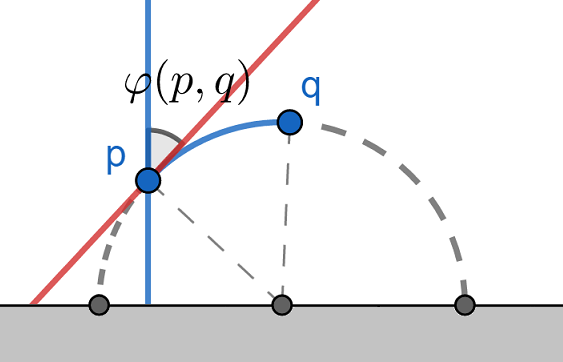
\includegraphics[width=0.5\textwidth]
  {figures/hyperbolic.png}

图:测地线$\ell(p,q)$、$\ell(p,\infty)$,以及夹角$\fai(p,q)$.
\end{figure}

事实上,由初等平面几何容易给出$\fai(p,q)$的显式表达式:
$$\fai(p,q)=\arg\left(\frac{q-\overline{p}}{q-p}\right)$$
以上出现的夹角、辐角可以取任意的分支。

\begin{notation}%Let
对于$n\geq 0$,定义
$$\Conf_n(\bbH):=\{(p_1,...,p_n)\in\bbH|
p_i\neq p_j,\,\forall i\neq j\}$$
则$\Conf_n(\bbH)$有自然的$2n$维光滑流形结构($\bbR^{2n}$的开子流形)。

%For each arrow in $\Gamma$,
对于图$\Gamma=(\Gma_0,\Gma_1,\veps)\in G_n$,
以及$e\in\Gma_1$,定义流形$\Conf_n(\bbH)$上的光滑函数$\fai_e$如下:
\begin{eqnarray*}
\fai_e:\Conf_n(\bbH)&\to&\bbR\\
(p_1,...,p_n)&\mapsto&\fai(p_{s(e)},p_{t(e)})
\end{eqnarray*}
其中特别规定$p_L=0\in\overline{\bbH}$,
以及$p_R=1\in\overline{\bbH}$
\end{notation}

粗俗地说,对于图$\Gma\in G_n$,
$\Conf_n(\bbH)$当中的一个元素$\bfp$可以视为
“将图$\Gma$嵌入双曲平面$\bbH$的一种方式”:
图$\Gma$的“一般顶点”的位置由$\bfp$给出,
“特殊顶点”$L,R$分别位于$0,1$;
图$\Gma$当中的边对应于$\bbH$中的测地线。
此时,$\fai_e$可以认为是边$e$的“倾斜角”。

\begin{definition}
对于图$\Gma\in G_n$,定义
$$
  \omg_{\Gamma}=\frac{1}{n!(2\pi)^{2n}}
  \int_{\Conf_n(\bbH)}
    \bigwedge_{i=1}^n(\td\fai_{a_i}\wedge\td\fai_{b_i})
$$
%check: it is convergent.
\end{definition}
这是$2n$-形式在$2n$-维流形上的积分。
但需要验证此积分的收敛性,这里从略。
注意积分号前的系数$\frac{1}{n!(2\pi)^{2n}}$
是精心挑选的,我们稍后给出解释。
%见Kontsevich的原始论文

现在,我们可以完整地陈述以下定理:
\begin{thm}(Kontsevich)

任意的泊松流形$(X,P)$都存在形变量子化,
并且星积可以由以下公式显式给出:%The formula
$$
  f\star g
=
  \sum_{n=0}^{\infty}
    \hbar^n
    \left(
      \sum_{\Gma\in G_n}
        \omg_{\Gma}
        B_\Gma(f,g)
    \right)
$$
%gives a deformation quantization of $P$
\end{thm}
在此述而不证。构造如此星积$\star$的动机、
想法,来自于量子场论等物理背景,我们在后文会介绍之。

\begin{example}($\omg_{\Gma}$最基本的显式计算)

我们考虑简单(但重要的)情形:$\Gma,\Gma'\in G_1$分别为如下:
$$
  \xymatrix{
    &1\ar[dl]_{a_1}  \ar[dr]^{b_1}
    &
  \\
     L
    &
    &R
  }
\quad
   \xymatrix{
    &1\ar[dl]_{b_1}  \ar[dr]^{a_1}
    &
  \\
     L
    &
    &R
  }
$$
那么有
$$\omg_\Gma=\frac{1}{2}\quad,\quad \omg_{\Gma'}=-\frac{1}{2}$$
\end{example}

\begin{proof}
我们只需要求$\omg_{\Gma}$,
而注意到$\Gma$与$\Gma'$的区别仅仅是两条边对换,
从而倾斜角$\fai_{\Gma,a_1}=\fai_{\Gma',b_1}$,
$\fai_{\Gma,b_1}=\fai_{\Gma',a_1}$,
再由外积的反对称性,容易观察出$\omg_{\Gma}=-\omg_{\Gma'}$.

现在计算$\omg_\Gma$.
此时$n=1$,$\Conf_1(\bbH)\cong H$,
对任意的$z=x+iy\in\bbH\cong\Conf_1(\bbH)$,
由初等几何容易知道
$$
  \begin{array}{ll}
    \fai_{a_1}(z)=-2\arg z\\
    \fai_{b_1}(z)=-2\arg(z-1)
  \end{array}
$$
(允许相差$2\pi$的整数倍,这无所谓)从而
$$
    \td\fai_{a_1}(z)=-2\td\arctan\left(\frac{y}{x}\right)
=-2\frac{x\td y-y\td x}{x^2+y^2}
$$
同理
$$\td\fai_{b_1}(z)=-2\frac{(x-1)\td y-y\td x}{(x-1)^2+y^2}$$
因此有
\begin{eqnarray*}
     \omg_\Gma
&=&
     \frac{1}{1!(2\pi)^{2\times1}}
     \int_{\Conf_1(\bbH)}
       \td\fai_{a_1}
       \wedge
       \td\fai_{b_1}\\
&=&
     \frac{1}{4\pi^2}
     \int_{\bbH}
       \frac{4y}
            {(x^2+y^2)\big((x-1)^2+y^2\big)}
       \td x\wedge\td y\\
&=&
     \frac{1}{\pi^2}
     \int_{0}^{\pi}
       \sin\theta
       \td\theta
     \int_0^{\infty}
       \frac{1}
            {r^2-2r\cos\theta+1}
       \td r\\
&=&
     \frac{1}{\pi^2}
     \int_{0}^{\pi}
       (\pi-\theta)
       \td\theta
=
     \frac{1}{2}
\end{eqnarray*}
\end{proof}

\begin{rem}
事实上,如果泊松张量的分量$P^{ij}$在局部上是常值的,
那么Kontsevich给出的量子化公式刚好是Moyal星积
(见例子\ref{Moyal星积-def}),
从而Kontsevich量子化$\star_K$是Moyal星积$\star_M$的推广。
回顾我们此前已经给出了Moyal星积的显式表达式
$$f\star_M g=\sum_{k=0}^{\infty}\frac{\hbar^k}{k!}
\sum_{|I|=|J|=k}P^{I,J}(\p_If)(\p_Jg)$$
\end{rem}

\begin{proof}
我们来考察$P^{ij}$为常数的情形。对于$n\geq 0$,以及$\Gamma\in G_n$,
注意到如果$\Gma$当中有箭头不指向$L$且不指向$R$,则双微分算子$B_\Gma$
当中含有对$P^ij$求导的项,因此$B_\Gma=0$,对$\star_K$没有贡献。
从而我们只需要考虑$G_n$的子集
$$\widetilde{G_n}:=\{\Gma\in G_n|t(a_i)\in\{L,R\},\forall 1\leq i\leq n\}$$
即,$\widetilde{G_n}$当中的图具有性质:每个箭头都指向$L$或者$R$;
并且容易知道$\widetilde{G_n}$当中有$2^n$个元素。
现在,
$$
  f\star_K g=
  \sum_{n=0}^{\infty}
    \hbar^n
    \sum_{\Gma\in\widetilde{G_n}}
      \omg_{\Gma}B_{\Gma}(f,g)
$$
再注意到,对于任意$\Gma,\Gma'\in\widetilde{G_n}$,都有
$$\omg_{\Gma}B_{\Gma}=\omg_{\Gma'}B_{\Gma'}$$
这是由于两个$1-$形式的外积具有反交换性,
以及泊松张量分量$P^{ij}$关于指标的反对称性。
从而我们不妨取$\widetilde{G_n}$中的代表元
$\Gma^n\in\widetilde{G_n}\subseteq G_n$,其中$\Gma^n$满足:
所有的边$a_i$都指向$L$,所有的边$b_i$都指向$R$.从而
\begin{eqnarray*}
  f\star_K g
&=&
  \sum_{n=0}^{\infty}
    \hbar^n
      2^n\omg_{\Gma^n}B_{\Gma^n}(f,g)\\
&=&
  \sum_{n=0}^{\infty}
    \hbar^n2^n
      \omg_{\Gma^n}
      (P^{a_1b_1}\cdots P^{a_nb_n})
      (\p_{a_1}\cdots\p_{a_n}f)
      (\p_{b_1}\cdots\p_{b_n}g)
\end{eqnarray*}
最后再注意到
\begin{eqnarray*}
     \omg_{\Gma^n}
&=&
     \frac{1}{n!(2\pi)^{2n}}
     \int_{\bbH^n}
       \bigwedge_{i=1}^n
         (
         \td\fai_{a_i}(z_i)\wedge
         \td\fai_{b_i}(z_i)
         )\\
&=&
     \frac{1}{n!(2\pi)^{2n}}
     \prod_{i=1}^n
       \left(
         \int_{\bbH}
           \td\fai_{a_i}(z_i)\wedge
           \td\fai_{b_i}(z_i)
       \right)\\
&=&
     \frac{(2\pi^2)^n}{n!(2\pi)^{2n}}
 =
     \frac{1}{n!2^n}
\end{eqnarray*}
因此Kontsevich量子化$\star_K$满足
\begin{eqnarray*}
  f\star_K g
&=&
  \sum_{n=0}^{\infty}
    \hbar^n2^n
      \frac{1}{n!2^n}
      (P^{a_1b_1}\cdots P^{a_nb_n})
      (\p_{a_1}\cdots\p_{a_n}f)
      (\p_{b_1}\cdots\p_{b_n}g)\\
&=&
     \sum_{n=0}^{\infty}
      \frac{\hbar^n}{n!}
      (P^{a_1b_1}\cdots P^{a_nb_n})
      (\p_{a_1}\cdots\p_{a_n}f)
      (\p_{b_1}\cdots\p_{b_n}g)\\
\end{eqnarray*}
这正是Moyal乘积的表达式。
\end{proof}



%\begin{rem}
%if $P^{ij}$ is constant, then this is Moyal product.
%(也就是说,这是Moyal pruduct 的推广)
%结合性很不显然2333333
%以后会解释这个公式的来历。物理背景+非交换技术....
%\end{rem}
\section{指标定理}
index theorem:

Symplectic case: $(X,\omg)$ symplectic mfd,
$P=\omg^{-1}$

Fedosov: a single geometric way to get deformation quantization and the classification by
$$\omg_{\hbar}=-\omg+\hbar\omg_1+\hbar^2\omg_2+\cdots$$
where
$$\omg_i\in H^2(X,\bbR)$$

\begin{definition}
 the trace map
$$\tau: c^{\infty}(X)\to \bbR\Ls{\hbar}$$
satisfying
$$\tau(f\star g)=\tau(g\star f)$$
$$\Longrightarrow \tau\in \HH^0(C^{\infty}(x)\fps{\hbar})$$

Fedosov/Nest Tsygar: canonical trace

such that
$$\tau(f)=\frac{1}{(2\pi\hbar)^n}
\int_X
  \frac{\omg^n}{n!}
  (f+O(\hbar))$$
\end{definition}

注意记号:
$$\HH^i(A):=H^i(A,A^*)$$


\begin{thm}(Fedosov/Nest-Tsygan)

$$\tau(1)=\int_X e^{w_{\hbar}/\hbar}\Ahat(X)$$
(algebraic index thm)
where $\Ahat$ is the genus of $X$,
$$\Ahat(X):=
\det\nolimits^{1/2}\frac{R/2}{\sinh(R/2)}$$
$R$ is the curvature of $T_X$.
\end{thm}

Goal: explain both 1 and 2 from

non-commutative Hochschild theory

quantum- field theory

%%%%现在开始正课,刚才的故事讲完了%%%

\section{量子场论基础}
\textbf{Some basis of QFT}

a physics system always consists of
$$\mcalS:\mcalE\to\bbR$$
where $\mcalE$ is the space of field( of infinity dimension)

$\mcalS$ : actional functional%作用量

Classical physics:
$$Cirt(\mcalS)=\{\delta s=0\}$$

Quantum physics:
$$\int_{\mcalE}\theta e^{i\mcalS/\hbar}$$
"path integral", $\theta$ is a function on $\mcalE$("observable").

\begin{example}
$$\mcalE= C^{\infty}(X)$$
$$\mcalS[\fai]=\int_X|\nabla\fai|^2\quad\fai\in C^{\infty}(X)$$
(scalar field theory)
$$\delta\mcalS=0\Longrightarrow\Delta\fai=0$$
\end{example}

\begin{example}
$$\mcalE=\{\text{connections on $E\to X$}\}$$
$$F_A=\td A+\frac{1}{2}[A,A]$$
curvature
$$YM[A]=\int_XF_A\wedge*F_A$$
is called Yang-Mills functional.
\end{example}

\begin{example}($\sigma$-module)
$$\mcalE=map(\Sigma,X)$$
...
\end{example}

\begin{example}(Gravity)
$$\mcalE=\{\text{metrics on $X$}\}$$
\end{example}
以上是四种很经典的例子。

Problem: How to construct
$$\int_{\mcalE}\theta e^{i\mcalS/\hbar}$$

We introduce a different method:BV method
(Batalin-Vilkovisky)

Philosophy: measure theory$\int_X\mapsto$ Homology theory.....

Calculus
$$\int_X:\Omg_X\updot\to\bbR$$
where $X$ is compact oriented manifold of dimension $n$,

Observe:
$$H^n_{DR}(X)=H^n(\Omg\updot,\td)\cong\bbR$$
$$\int_X:\Omg^n\to H^n_{DR}\cong\bbR$$
$$\alpha\mapsto[\alpha]$$

$$\rightsquigarrow\int_X=H_{DR}^n$$
$$(\Omg\updot(X),\td)\rightsquigarrow\text{measure}$$

Question:how to $\int_X=H^n\quad n\to\infty$?

%%%%%%%%%%%%%%%%%%%%%%%%%%%%%%%%%%%%%%%%%%%%%%%%%%%%%%%%%
%%%%%%%%%%%%%%%%2019.3.26星期二 第五周%%%%%%%%%%%%%%%%%%%
%%%%%%%%%%%%%%%%%%%%%%%%%%%%%%%%%%%%%%%%%%%%%%%%%%%%%%%%%

%讲一些物理想法

\textbf{Feynman Diagram}

recall:
$$D^n_{DR}=\int_X:\Omg\updot(X)\to\bbR$$
what if $n\to \infty$?

Different philosophy:

Let $\PV\updot(X):=\Gamma(X,\wedgeform{*}TX)$,
$\Omg$ be a volume form($n$-form) on $X$,then
$$f\mapsto\int_Xf\Omg$$

$$\PV^k(X)\xra{\dashv\Omg}\Omg^{n-k}(X)$$
is a 1-1 coorespondence.
%%%%缩并%%%%%%%

$$\PV^*(X)\leftrightarrow \Omg^{n-\bullet}(X)$$
$$\yc\leftrightarrow \td$$
this "$\yc$" is called "divergence operator w.r.t the volume form".
when $x\in\PV^1(X)$,check: $\yc(v)=\div_{\Omg}v$.

$$\td^2=0\Rightarrow\yc^2=0$$

$$\PV^n\xra{\yc}\PV^{n-1}\xra{\yc}\PV^{n-2}\to\cdots$$
$\yc$ is also called "BV operator".

$$\int_{BV}:=H_0(\yc)$$
good news: $0$ doesn't depend on $\dim(X)$!
(so, we can $n\to\infty$???)

\textbf{Difficulty}: when $n\to\infty$, we need to construct $\yc$.

\begin{example}
Let $X$ is a manifold of finite dimension, $\dim X=n$,
local coordinate $\{x^1,...,x^n\}$ in $\mcalU\subseteq X$,
volume form
$$\Omg=e^{f(x)}\td x^1\wedge\cdots\wedge\td x^n$$

$$\Omg\updot(\mcalU):=C^{\infty}(\mcalU)[\td x^1,...,\td x^n]$$
where $\td x^i\wedge\td x^j=-\td x^j\wedge\td x^i$.

$\PV\updot(\mcalU):=C^{\infty}(\mcalU)[\p_1,...,\p_n]$
 where $\p^i\wedge\p^j=-\p^j\wedge\p^i$.
\end{example}

introduce grassman variables $\theta_1,...,\theta_n$,
($\theta _i\cong \p_i$)

define
$$\PV\updot(\mcalU):=C^{\infty}(\mcalU)[\theta_1,...,\theta_n]$$

%%%%%%%非交换的微积分%%%%%%%%

\begin{prop}
$$\Omg=e^{f(x)}\td x^1\wedge\cdots\wedge \td x^n$$
$$\PV=C^{\infty}(u)[\theta_1,...,\theta_n]$$
then

$$\yc_{\Omg}=\sum_{i}\pp{x^i}\pp{\theta_i}
-\sum_{i}\p_if(x)\pp{\theta_i}$$

(Odd Laplacian)
(这是BV算子的等价定义。。。)
\end{prop}

\begin{proof}
%笔记里找
\end{proof}


\begin{definition}
Given $\yc_{\Omg}$(BV operator), we define
$$\{,\}:\PV\times\PV\to\P$$
$$\{\alpha,\beta\}:=
\yc_{\Omg}(\alpha\wedge\beta)-(\yc_{\Omg}\alpha)\wedge\beta-
(-1)^{|\alpha|}\alpha\wedge\yc_{\Omg}\beta$$
the failure of $\yc_{\Omg}$ being a derivation.
\end{definition}
Check: $\{,\}$ is a Schouten-Nijenhuis bracket(up to sign).
(independent of the choice of $f(x)$)

In particular,$\{,\}$ is independent of choice of $\Omg$.

\textbf{Quantization}

$$\{,\}\xra{?}\yc_{\Omg}$$
这个过程与量子化的过程是一样的??WTF??

\textbf{Feymann Diagram}
\begin{example}
$X=\bbR$,
$$\Omg=\frac{1}{\sqrt{2\pi}}e^{-\frac{1}{2}x^2}\td x$$
$$\int:\bbR[x]\to\bbR$$
$$g\mapsto\int_{\bbR}g\Omg$$

$\PV=\bbR[x,\theta]$, and
$$\yc_{\Omg}=\pp{x}\pp{\theta}-x\pp{\theta}$$
%符号可能不对,小心check

$$\int_{BV}:\bbR[x,\theta]\mapsto H^0(\yc_{\Omg})$$

if $g=g(x)$, then $\yc_{\Omg}g=0$. Let $[g]$ be the
$\yc_{\Omg}$- homology class,
$$\yc_{\Omg}(x^{m-1}\Omg)
=(m-1)x^{m-2}
-x^m$$
$$\Rightarrow [x^m]=(m-1)[x^{m-2}]$$
so,
$$
[x^m]=
\left\{
  \begin{array}{cc}
    0  &  m \text{ is odd}\\
    (2k-1)!![1]  & m=2k
  \end{array}
\right.
$$

so,
$$\int_{\bbR}x^{2k}\Omg=
(2k-1)!!\int_{\bbR}\Omg=(2k-1)!!$$

\end{example}

introduce the operator
$$\mcalU:=
  e^{\frac{1}{2}\pp{x}\pp{x}}:
  \bbR[x,\theta]\to\bbR[x,\theta]
$$

\begin{lemma}
$$\yc_{\Omg}=\mcalU^{-1}(-x\pp{\theta})\mcalU$$
\end{lemma}
\begin{proof}
use the formula
$$e^ABe^{-A}=e^{\ad_A}B$$
then
$$\yc_{\Omg}=\pp{x}\pp{\theta}-x\pp{\theta}
$$
$$A=-\frac{1}{2}\pp{x}\pp{x}$$
$$B=-x\pp{\theta}$$
then
$$e^ABe^{-A}=\pp{x}\pp{\theta}$$
where $[A,[A,B]]=0$.
\end{proof}

so,
$$\mcalU\circ\yc_{\Omg}=(-x\pp{\theta})\circ\mcalU$$

so,
$$\mcalU:(\bbR[x,\theta,\yc_{\Omg}])\to
(\bbR[x,m\theta],-x\pp{\theta})$$
is a co-chain map.

$$H\updot(\bbR[x,\theta],-x\pp{\theta})$$
$$\bbR[x]\theta\xra{-x\pp{\theta}}\bbR[x]$$
$$g\mapsto -xg(0)$$
$H^{-1}=0$,$H^0=\bbR$.

$$\mcalU[g(x)]_{\yc_{\Omg}}=[\mcalU(g)(x)]_{-x\pp{\theta}}
=[\mcalU(g)(0)]_{-x\pp{\theta}}
=\mcalU(g)(0)[1]$$

so,
$$\int_{\bbR}g(x)\Omg=\mcalU(g)(0)=
e^{\frac{1}{2}\pp{x}\pp{x}}|_{x=0}g(x)$$

More generally, check:
$$\int_{\bbR}g(x+a)\Omg=
e^{\frac{1}{2}\pp{x}\pp{x}}|_{x=a}g(x)$$


\begin{example}
Consider the integral
$$
  \int_{\bbR}
    e^{(-\frac{1}{2}x^2+\frac{1}{3!}x^3)/\hbar}
    \frac{\td x}{\sqrt{2\pi\hbar}}
$$
this integral is not convergent.... how to deal with it?

(1)Change the integration Contour inside $\bbC$
%%%%%%%Contour%%%%%%%
(Airy function)

(2)We consider only the asymptotic series
$$
  \sum_{n\geq 0}\frac{1}{n!}
    \int
      \left(
        \frac{\lmd x^3}{3!\hbar}^n
      \right)
      e^{-\frac{1}{2}x^2/\hbar}
      \frac{\td x}{\sqrt{2\pi\hbar}}
$$

$$\yc_{Omg}=\hbar\pp{x}\pp{\theta}-x\pp{\theta}$$
$$\mcalU_{\hbar}=e^{\frac{\hbar}{2}\pp{x}\pp{x}}$$
then

%%%%%%%%微积分%%%%%%%%%
introduce graph with cubic vertex,

each edge: we put $\hbar\pp{a}\pp{a}$

each point: we put $\frac{\lmd a^3}{3!\hbar}$

$$\omg_{\gamma}(a)$$
by the above rule.

%%%%%%这又是什么图%%%%%%%
\end{example}

\begin{thm}(Feymann graph formula)

this integration is
$$
   \int_{\bbR}
     e^{(-\frac{1}{2}x^2+\frac{\lmd}{3}(x+a)^3)/\hbar}
     \frac{\td x}{\sqrt{2\pi\hbar}}
=
   \sum_{\Gamma:\text{trivalent graphs}}
     \frac{w_{\Gamma}(a)}
          {|\text{Aut}(\gamma)|}
=
   \sum
$$
\end{thm}
\begin{proof}
check.
\end{proof}

In general, consider









